\documentclass[conference]{IEEEtran}
% \documentclass[conference]{../sty/IEEEtran}

% *** CITATION PACKAGES ***
%
%\usepackage{cite}
% cite.sty was written by Donald Arseneau
% V1.6 and later of IEEEtran pre-defines the format of the cite.sty package
% \cite{} output to follow that of the IEEE. Loading the cite package will
% result in citation numbers being automatically sorted and properly
% "compressed/ranged". e.g., [1], [9], [2], [7], [5], [6] without using
% cite.sty will become [1], [2], [5]--[7], [9] using cite.sty. cite.sty's
% \cite will automatically add leading space, if needed. Use cite.sty's
% noadjust option (cite.sty V3.8 and later) if you want to turn this off
% such as if a citation ever needs to be enclosed in parenthesis.
% cite.sty is already installed on most LaTeX systems. Be sure and use
% version 5.0 (2009-03-20) and later if using hyperref.sty.
% The latest version can be obtained at:
% http://www.ctan.org/pkg/cite
% The documentation is contained in the cite.sty file itself.

% *** GRAPHICS RELATED PACKAGES ***
%
\ifCLASSINFOpdf
   \usepackage[pdftex]{graphicx}
  % declare the path(s) where your graphic files are
  % \graphicspath{{../pdf/}{../jpeg/}}
  % and their extensions so you won't have to specify these with
  % every instance of \includegraphics
  % \DeclareGraphicsExtensions{.pdf,.jpeg,.png}
\else
  % or other class option (dvipsone, dvipdf, if not using dvips). graphicx
  % will default to the driver specified in the system graphics.cfg if no
  % driver is specified.
   \usepackage[dvips]{graphicx}
  % declare the path(s) where your graphic files are
  % \graphicspath{{../eps/}}
  \graphicspath{ {./img/} }
  % and their extensions so you won't have to specify these with
  % every instance of \includegraphics
  % \DeclareGraphicsExtensions{.eps}
\fi
\graphicspath{ {./img/} }
% graphicx was written by David Carlisle and Sebastian Rahtz. It is
% required if you want graphics, photos, etc. graphicx.sty is already
% installed on most LaTeX systems. The latest version and documentation
% can be obtained at: 
% http://www.ctan.org/pkg/graphicx
% Another good source of documentation is "Using Imported Graphics in
% LaTeX2e" by Keith Reckdahl which can be found at:
% http://www.ctan.org/pkg/epslatex
%
% latex, and pdflatex in dvi mode, support graphics in encapsulated
% postscript (.eps) format. pdflatex in pdf mode supports graphics
% in .pdf, .jpeg, .png and .mps (metapost) formats. Users should ensure
% that all non-photo figures use a vector format (.eps, .pdf, .mps) and
% not a bitmapped formats (.jpeg, .png). The IEEE frowns on bitmapped formats
% which can result in "jaggedy"/blurry rendering of lines and letters as
% well as large increases in file sizes.
%
% You can find documentation about the pdfTeX application at:
% http://www.tug.org/applications/pdftex

% *** MATH PACKAGES ***
%
%\usepackage{amsmath}
% A popular package from the American Mathematical Society that provides
% many useful and powerful commands for dealing with mathematics.
%
% Note that the amsmath package sets \interdisplaylinepenalty to 10000
% thus preventing page breaks from occurring within multiline equations. Use:
%\interdisplaylinepenalty=2500
% after loading amsmath to restore such page breaks as IEEEtran.cls normally
% does. amsmath.sty is already installed on most LaTeX systems. The latest
% version and documentation can be obtained at:
% http://www.ctan.org/pkg/amsmath


% *** SPECIALIZED LIST PACKAGES ***
%
\usepackage{algorithmic}
% algorithmic.sty was written by Peter Williams and Rogerio Brito.
% This package provides an algorithmic environment fo describing algorithms.
% You can use the algorithmic environment in-text or within a figure
% environment to provide for a floating algorithm. Do NOT use the algorithm
% floating environment provided by algorithm.sty (by the same authors) or
% algorithm2e.sty (by Christophe Fiorio) as the IEEE does not use dedicated
% algorithm float types and packages that provide these will not provide
% correct IEEE style captions. The latest version and documentation of
% algorithmic.sty can be obtained at:
% http://www.ctan.org/pkg/algorithms
% Also of interest may be the (relatively newer and more customizable)
% algorithmicx.sty package by Szasz Janos:
% http://www.ctan.org/pkg/algorithmicx


% *** ALIGNMENT PACKAGES ***
%
%\usepackage{array}
% Frank Mittelbach's and David Carlisle's array.sty patches and improves
% the standard LaTeX2e array and tabular environments to provide better
% appearance and additional user controls. As the default LaTeX2e table
% generation code is lacking to the point of almost being broken with
% respect to the quality of the end results, all users are strongly
% advised to use an enhanced (at the very least that provided by array.sty)
% set of table tools. array.sty is already installed on most systems. The
% latest version and documentation can be obtained at:
% http://www.ctan.org/pkg/array


% IEEEtran contains the IEEEeqnarray family of commands that can be used to
% generate multiline equations as well as matrices, tables, etc., of high
% quality.




% *** SUBFIGURE PACKAGES ***
%\ifCLASSOPTIONcompsoc
%  \usepackage[caption=false,font=normalsize,labelfont=sf,textfont=sf]{subfig}
%\else
%  \usepackage[caption=false,font=footnotesize]{subfig}
%\fi
% subfig.sty, written by Steven Douglas Cochran, is the modern replacement
% for subfigure.sty, the latter of which is no longer maintained and is
% incompatible with some LaTeX packages including fixltx2e. However,
% subfig.sty requires and automatically loads Axel Sommerfeldt's caption.sty
% which will override IEEEtran.cls' handling of captions and this will result
% in non-IEEE style figure/table captions. To prevent this problem, be sure
% and invoke subfig.sty's "caption=false" package option (available since
% subfig.sty version 1.3, 2005/06/28) as this is will preserve IEEEtran.cls
% handling of captions.
% Note that the Computer Society format requires a larger sans serif font
% than the serif footnote size font used in traditional IEEE formatting
% and thus the need to invoke different subfig.sty package options depending
% on whether compsoc mode has been enabled.
%
% The latest version and documentation of subfig.sty can be obtained at:
% http://www.ctan.org/pkg/subfig



% *** FLOAT PACKAGES ***
%
%\usepackage{fixltx2e}
% fixltx2e, the successor to the earlier fix2col.sty, was written by
% Frank Mittelbach and David Carlisle. This package corrects a few problems
% in the LaTeX2e kernel, the most notable of which is that in current
% LaTeX2e releases, the ordering of single and double column floats is not
% guaranteed to be preserved. Thus, an unpatched LaTeX2e can allow a
% single column figure to be placed prior to an earlier double column
% figure.
% Be aware that LaTeX2e kernels dated 2015 and later have fixltx2e.sty's
% corrections already built into the system in which case a warning will
% be issued if an attempt is made to load fixltx2e.sty as it is no longer
% needed.
% The latest version and documentation can be found at:
% http://www.ctan.org/pkg/fixltx2e


%\usepackage{stfloats}
% stfloats.sty was written by Sigitas Tolusis. This package gives LaTeX2e
% the ability to do double column floats at the bottom of the page as well
% as the top. (e.g., "\begin{figure*}[!b]" is not normally possible in
% LaTeX2e). It also provides a command:
%\fnbelowfloat
% to enable the placement of footnotes below bottom floats (the standard
% LaTeX2e kernel puts them above bottom floats). This is an invasive package
% which rewrites many portions of the LaTeX2e float routines. It may not work
% with other packages that modify the LaTeX2e float routines. The latest
% version and documentation can be obtained at:
% http://www.ctan.org/pkg/stfloats
% Do not use the stfloats baselinefloat ability as the IEEE does not allow
% \baselineskip to stretch. Authors submitting work to the IEEE should note
% that the IEEE rarely uses double column equations and that authors should try
% to avoid such use. Do not be tempted to use the cuted.sty or midfloat.sty
% packages (also by Sigitas Tolusis) as the IEEE does not format its papers in
% such ways.
% Do not attempt to use stfloats with fixltx2e as they are incompatible.
% Instead, use Morten Hogholm'a dblfloatfix which combines the features
% of both fixltx2e and stfloats:
%
% \usepackage{dblfloatfix}
% The latest version can be found at:
% http://www.ctan.org/pkg/dblfloatfix




% *** PDF, URL AND HYPERLINK PACKAGES ***
%
%\usepackage{url}
% url.sty was written by Donald Arseneau. It provides better support for
% handling and breaking URLs. url.sty is already installed on most LaTeX
% systems. The latest version and documentation can be obtained at:
% http://www.ctan.org/pkg/url
% Basically, \url{my_url_here}.

\usepackage[utf8]{inputenc}
\usepackage{amssymb}
\usepackage{algorithm}
\newtheorem{definition}{Definition}
\renewcommand{\algorithmicrequire}{\textbf{Input:}}
\renewcommand{\algorithmicensure}{\textbf{Output:}}

\newcommand\alberto[1]{\textcolor{black}{#1}}

% *** Do not adjust lengths that control margins, column widths, etc. ***
% *** Do not use packages that alter fonts (such as pslatex).         ***
% There should be no need to do such things with IEEEtran.cls V1.6 and later.
% (Unless specifically asked to do so by the journal or conference you plan
% to submit to, of course. )


% correct bad hyphenation here
\hyphenation{op-tical net-works semi-conduc-tor}

\begin{document}
%
% paper title
% Titles are generally capitalized except for words such as a, an, and, as,
% at, but, by, for, in, nor, of, on, or, the, to and up, which are usually
% not capitalized unless they are the first or last word of the title.
% Linebreaks \\ can be used within to get better formatting as desired.
% Do not put math or special symbols in the title.
\title{You are the way you structurally talk: structural-temporal neighbourhoods of posts to characterize users in online forums}


% author names and affiliations
% use a multiple column layout for up to three different
% affiliations
\author{\IEEEauthorblockN{Alberto Lumbreras \\ Julien Velcin}
\IEEEauthorblockA{Laboratoire ERIC\\ Université de Lyon, France\\
alberto.lumbreras@univ-lyon2.fr\\
julien.velcin@univ-lyon2.fr}
\and
\IEEEauthorblockN{Bertrand Jouve}
\IEEEauthorblockA{FRAMESPA/IMT\\Université de Toulouse 2, France\\
jouve@univ-tlse2.fr}
\and
\IEEEauthorblockN{Marie Guégan}
\IEEEauthorblockA{Technicolor, France\\
marie.guegan@technicolor.com}}


% conference papers do not typically use \thanks and this command
% is locked out in conference mode. If really needed, such as for
% the acknowledgment of grants, issue a \IEEEoverridecommandlockouts
% after \documentclass

% for over three affiliations, or if they all won't fit within the width
% of the page, use this alternative format:
% 
%\author{\IEEEauthorblockN{Alberto Lumbreras\IEEEauthorrefmark{1},
%Bertrand Jouve\IEEEauthorrefmark{2},
%Marie Guégan\IEEEauthorrefmark{3}, 
%Julien Velcin\IEEEauthorrefmark{4}}
%\IEEEauthorblockA{\IEEEauthorrefmark{1}Technicolor, France\\Email: alberto.lumbreras@gmail.com}
%\IEEEauthorblockA{\IEEEauthorrefmark{2}Université de Toulouse; UT2; FRAMESPA/IMT,\\ 5 allée Antonio Machado, 31058 Toulouse, cedex 9\\
%Email: jouve@univ-tlse2.fr}
%\IEEEauthorblockA{\IEEEauthorrefmark{3}Technicolor\\975 Avenue des Champs Blancs\\35576 Cesson-Sevigné,\\France\\Email: marie.guegan@technicolor.com}
%\IEEEauthorblockA{\IEEEauthorrefmark{4}Laboratoire ERIC, Université de Lyon,\\ 5 avenue Pierre Mendès France, 69676, Bron\\France\\Email: julien.velcin@univ-lyon2.fr}}

% use for special paper notices
\IEEEspecialpapernotice{(Draft version: \today)}

% make the title area
\maketitle

% As a general rule, do not put math, special symbols or citations
% in the abstract
\begin{abstract}Users of social networks are often characterised by extracting some relevant features from the graphs associated to that network. The structural dynamic of the conversation are usually forgotten due to a lack of proper tools. We present a purely graph-based method to cluster users in online forums. 
\end{abstract}

% no keywords




% For peer review papers, you can put extra information on the cover
% page as needed:
% \ifCLASSOPTIONpeerreview
% \begin{center} \bfseries EDICS Category: 3-BBND \end{center}
% \fi
%
% For peerreview papers, this IEEEtran command inserts a page break and
% creates the second title. It will be ignored for other modes.
\IEEEpeerreviewmaketitle



\section{Introduction}
The interactions between users in online forums are often modelled as complex networks. As such, they can be studied from many levels, each of which is represented by a graph where vertices and edges may represent different things. The most studied graph is a graph where vertices represent users and edges represent interactions between users (a post from one user replying to a post from other user). From the point of view of the community, some typically analysed properties are the degree distribution, the clustering coefficient, density, or diameter of the graph. From the point of view of the individual users, analyses are typically focused either on the centrality of users, on the community structure or in blockmodeling (groups of users that tend to interact with the same other groups) \cite{McCallum2007a}. Another common graph is a tree graph where vertices represent posts (or e-mails) and and edges from one vertex to another indicates that the first is a reply to the second. Given the different discussion trees of a forum (a forest) the global analyses include the depth distribution, branching factors, or even the time between two posts \cite{Bhatt2012}. representation include depth distribution of discussions, branching factors and so. Studying discussion trees from the point of view of the users means, since trees are discussions, studying the user at a conversational level. Unfortunately, there is a lack of structural tools to perform this analysis. In this paper, we propose to fill this gap through the concept of \textit{structural-temporal neighbourhood}.  
%El esquema debe ser;
%- SNA: 
%*** comunidad: degree distribution, density, clustering coefficient etc
%*** usuario: centrality
%- Tree/forest:
%*** global properties: degree distribution, depth distribution, inter-message times,...
%** Individual properties: ... 

Our goal in this paper is two-fold: on the one hand, to illustrate how structural-temporal neighbourhoods can play the role of triads for conversation trees, in the sense that they show us the local structures or dynamics from which the bigger graph emerges. On the other hand, to show how structural-temporal neighbourhoods can be used for the detection of different types of conversationalists in online forums or any other type of online discussion that is representable by a tree structure (e.g.: e-mails).

The remaining of the paper is as follows. We first discuss about the convenience of the classic neighbourhood definition in dynamic graphs such as discussion trees. Then we introduce our two definitions of structural-temporal neighbourhoods. To illustrate the kind of neighbourhoods that we obtain in a real data, we analyse the neighbourhood census of a Reddit forum. Finally, we apply both neighbourhood definitions to detect clusters of users that tend to appear in the same neighbourhoods. We close the paper with some suggestions of future research.
%\begin{figure}
%	\centering
	%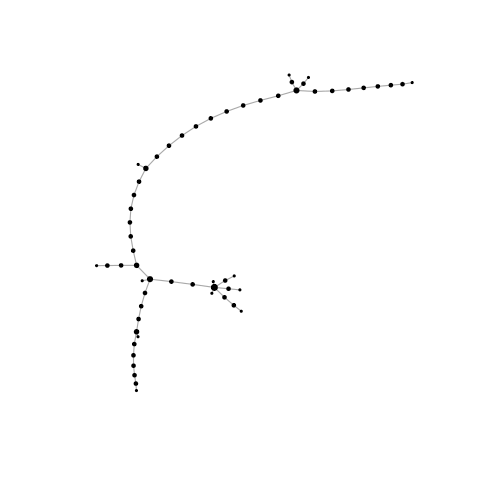
\includegraphics[width=0.3\textwidth]{tree1}
%	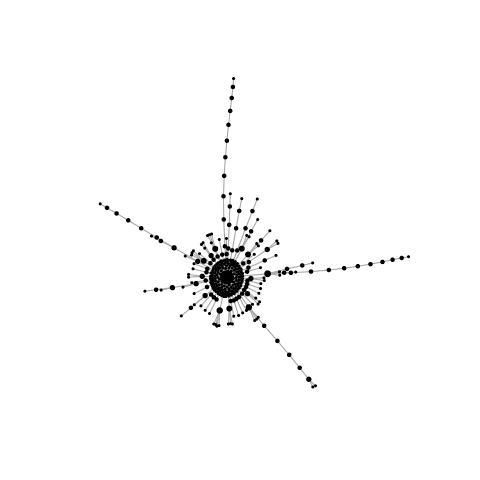
\includegraphics[width=0.3\textwidth]{tree2}
	%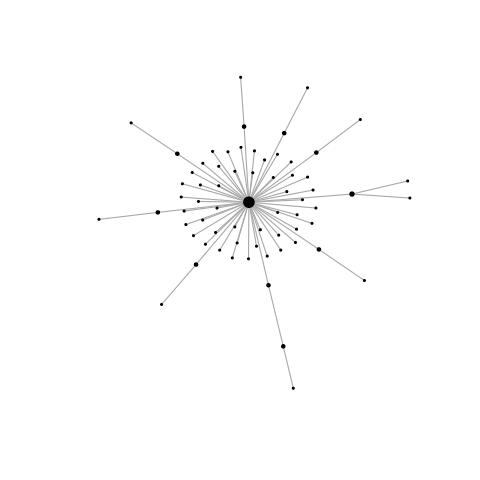
\includegraphics[width=0.3\textwidth]{tree3}
%	\caption{Representation of discussion threads with post tree graphs. Vertex represent posts and edges represent replies between posts.}
%	\label{fig:trees}
%\end{figure}

\section{Discussion trees}
% Introduce el objeto y la nomenclatura
We represent a discussion thread by a tree graph $G=(V,E)$ where $V$ is a set of $n$ vertices representing the posts (also called messages or comments) and $E$ is a set of $n-1$ directed edges that say which posts replied to which post. Vertices have two attributes namely time and author. If for two given vertices $v_i,v_j$ there exists an edge  $e=(v_i, v_j) \in E$ then $v_j$ is called the \textit{parent} of $v_i$, denoted as $p(v_i)=v_j$. The \textit{root} of the tree is the only vertex with no parent, and corresponds to the post that starts the discussion. We say that two vertices $v_i,v_j$ are \textit{siblings} if and only if $p(v_i)=p(v_j)$. A vertex $v_i$ is an ancestor of a vertex $v_j$ and $v_j$ is descendant of $v_i$ if and only if $v_i$ is in the path from $v_j$ to the root. A \textit{leaf} is a post with no replies. A \textit{branch} is the path between a leaf and the root. Two vertices $v_i$ and $v_i$ are said to be \textit{neighbours} if either $p(v_i)=v_j$ or $p(v_j)=v_i$ or, in other words, if their distance in the undirected version of $G$ is one.

%The interactions like those found in an online forum can be modelled, at least, by two sort of graphs. On the one hand, we can create a graph where vertices represent individuals and an edges represent an interaction between two individuals. At the individual level, this graph is suitable for a large set of analysis concerning the centrality of users, the detection of communities, the detection of groups that tend to interact with the same other groups. At the community level we can analyse properties such as the density of the graph, the clustering coefficient or the degree distribution. On the other hand, we can create a separate tree graph for every discussion where posts are represented by the vertices and and edge from one vertex to another indicates that first post is a reply to the second. This allows to analyse things like patterns of time delay between posts \cite{Bhatt2012}.

%We can even mix different levels of representations to study the relationship between the properties and dynamics among the different levels \cite{Dorat2007}.

%Of course, we are not limited to the study of graphs and some studies take into account the content of the conversations, the cross-posting activity of users, and so forth \cite{Whittaker1998}

%Others: \cite{Gaumont2016}

\section{Structural neighbourhoods}
Extending the classic definition of neighbourhood according to which two vertices are neighbours if the distance between them is one, we start by the following definition of \textit{structural neighbourhood}:

\begin{definition}
Given a tree graph $G$, the \textit{structural neighbourhood} of radius $r$ of post $i$, denoted as $\mathcal{N}_i(r)$, is the induced graph composed of all the vertices that are at distance equal or less than $r$ from post $i$.
\end{definition}
% pros and cons
In the context of discussion threads, this definition has two limitations. First, the decision on whether to include some post in the neighbourhood is only based on the structural distance, and therefore two posts that are at distance $d\leq r$ are considered neighbours of $i$ regardless of the time when they were written. In conversations, time plays an important role, therefore this is an important limitation. Another consequence of looking only at the structure is that the number of possible neighbourhoods within a radius $r$ is infinite. This poses a problem when trying to categorize conversations since many conversations, while structurally different, can be considered semantically equivalent.

\section{Structural-temporal neighbourhoods}
As we have discussed, structural neighbourhood falls short in the analysis of conversational structures. Instead, we propose two new definitions of neighbourhood that take into account the order and time in which posts are written. 

\begin{figure*}
\centering
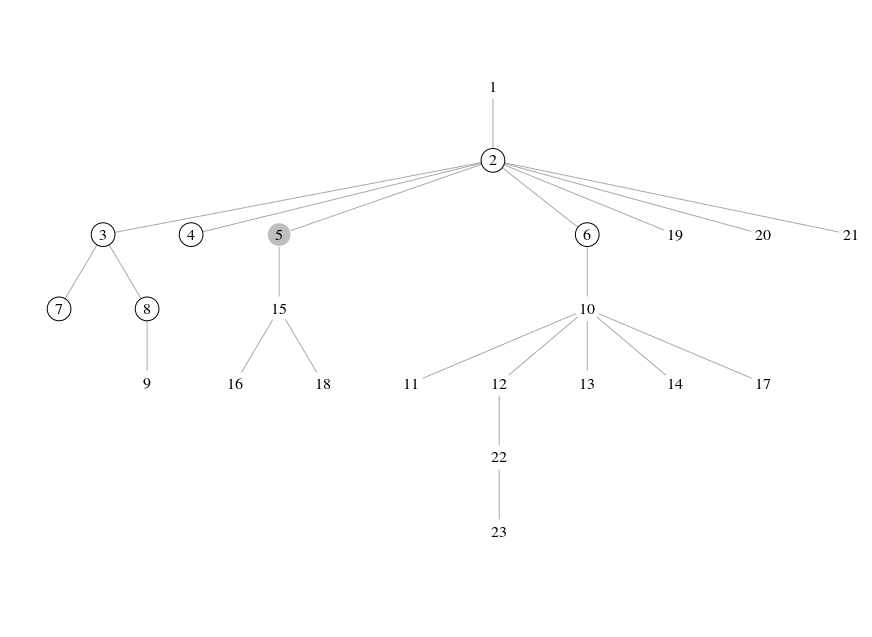
\includegraphics[width=0.45\textwidth]{order_neighbourhood}
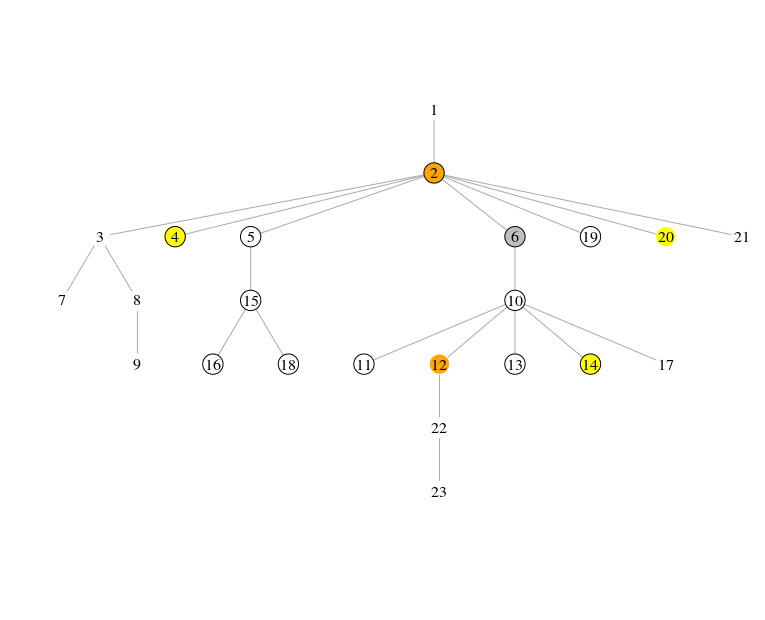
\includegraphics[width=0.45\textwidth]{breakpoints}
\caption{Illustration of order-based (left) and time-based (right) neighbourhoods. Grey nodes represent the ego post. Nodes with circles are those in the neighbourhood. Numbers indicate the order of the post. The order-based neighbourhood has parameters $r=3$, $n=6$. In the time-based neighbourhood, horizontal changepoints (yellow) and vertical changepoints (orange) represent posts that are temporally far from their predecessors (siblings or parents) and therefore set the limits of the neighbourhood.}
\label{fig:cutpoints}
\end{figure*}
\subsection{Order-based}
Our first definition is based on the order in which posts are attached to the tree. 
\begin{definition}
Given a ordered tree graph $G$, the \textit{order-based neighbourhood} of radius $r$ of vertex $i$, denoted as $\mathcal{N}_{i}^T(r,n)$ is the induced subgraph from its structural neighbourhood composed the $n$ vertices that are closest to $i$ in time and for which there exists a path to $i$ in $\mathcal{N}_{i}^T(r,n)$.  
\end{definition}
An example of order-based neighbourhood is given in Figure~\ref{fig:cutpoints} (left).
This definition has two advantages over the \textit{structural neighbourhood}. First, the temporal aspect of the conversation is better taken into account since the neighbourhood only includes posts that are not only near to $i$ in the structure but also in time. Second, the size of the neighbourhood has an upper bound of $min(|\mathcal{N}_i(r))|, n)$ thus making the space of possible neighbourhood structures finite. The main limitation of this definition is that the obtained neighbourhoods might be very different with different choices of $r$ and $n$, and we have no \textit{a priori} criteria to choose the proper parameters other than making them small so that the neighbourhoods capture the local dynamic of the conversation around the post $i$.

\subsection{Time-based}
In a first attempt to take time into account, one might set fixed time-based boundaries for the neighbourhood and include only those posts whose timestamp $t_j$ is at distance less than $\tau$ from the ego post $i$, $|t_j-t_i|<\tau$. However, the pace at which posts are added to the conversation may be very different between conversation threads (and also within a thread) and we have no \textit{a priori} criteria for a proper choice of $\tau$. 

Rather than looking for a fixed time radius, we may look at changes in the pace how new posts are added to the thread. In statistical analysis, a \textit{changepoint} in a sequence $x_1,...x_n$ is a point that comes from a different probability distribution than its precedent values. If sequences are timestamps, they are monotonic increasing, therefore the changepoints will correspond to sudden pauses in the conversation. If applied either to the timestamps of posts in a branch (vertical sequence) or to the timestamps of the replies to the same post (horizontal sequence), we say that a sequence posts with timestamps $t_1,...,t_n$ belong to the same (vertical or horizontal) \textit{local dynamic} if there is no changepoint $t_i$ in the sequence such that $1 < i \leq n$. For the detection of changepoints we use the PELT algorithm \cite{Killick2012}\footnote{An implementation of this algorithm written by its own authors is available in the R library \texttt{changepoint}.}. Now we can introduce our second definition of neighbourhood.
\begin{definition}
Given a tree graph $G$, the \textit{time-based neighbourhood} of vertex $i$, denoted as $\mathcal{N}_{i}^T(r)$, is the maximal subgraph of the structural neighbourhood $\mathcal{N}_i(r)$ where all the vertices  belong to the same vertical and horizontal local dynamic than $i$.
\end{definition}
Note that we still have a radius parameter $r$ to guarantee that the resulting structure remains local even if no changepoint is detected near the post $i$. 

% Explain algorithm
Algorithm \ref{alg:temporal_neighbourhood} extracts time-based neighbourhoods of a given post according to the given definition. Since the breakpoints only depend on the tree and not on the particular post we analyse, we previously detect the horizontal and vertical breakpoints in the tree. In the case of multiple branches with some common posts, we consider that a common post is a vertical breakpoint if it is a vertical breakpoint in any of the branches. Once we have the breakpoints we can proceed with the algorithm. First, we extract the structural-neighbourhood. The time-based neighbourhood will be a subset of the later. Then, we look for horizontal and vertical breakpoints, which mark the frontiers of the time-based neighbourhood. There are four possible cases:

\begin{itemize}
\item A \textit{vertical breakpoint in the ancestors}:  If the breakpoint is in the path between the post and the root, then the breakpoint started the new local dynamic to which the ego post belongs. Thus, we remove the ancestors of the breakpoint, but not the breakpoint.
\item A  \textit{vertical breakpoint in the descendants}: If the breakpoint is a descendant then it started a new different dynamic and therefore we must remove the descendants of the breakpoint and the breakpoint itself. 
\item An \textit{horizontal breakpoint either in the older siblings or in the ancestors}: If the breakpoint is among the older siblings, then it started the horizontal dynamic to which the ego post belongs. Similarly, if the breakpoint is among the ancestors, then every older sibling of the breakpoint belongs to a previous local dynamic. In both cases, we remove the older siblings of the breakpoint but not the breakpoint.
\item An \textit{horizontal breakpoint elsewhere}: In any other case, the horizontal breakpoint starts a different local dynamic and therefore we remove its younger siblings and the breakpoint. 
\end{itemize}
Any time a vertex is remove we also remove its descendants. The final neighbourhood will be connected induced subgraph from the structural neighbourhood. If there are no changepoints in the structural neighbourhood, the time-base neighbourhood will be exactly the structural neighbourhood.

%Example
An example of time-based neighbourhood is given in Figure~\ref{fig:cutpoints} (right).

\begin{algorithm}[H]
\begin{algorithmic}
\REQUIRE Posts tree $g$, vertical breakpoints, horizontal breakpoints, ego post $ego$
\ENSURE Subgraph of $g$ with all vertices in $V(g)$
\STATE Compute structural neighbourhood $\mathcal{N}_i(r)$
\STATE ancestors $\leftarrow$  ancestors(ego) in $\mathcal{N}_i(r)$
\STATE older\_siblings $\leftarrow$ older\_siblings(ego) in $\mathcal{N}_i(r)$
\STATE dump $\leftarrow \varnothing$
\FOR{bp $\in$ vertical breakpoints}
 \IF{bp $\in$ ancestors}
   \STATE dump $\leftarrow$ dump $\cup$ ancestors(bp)
 \ELSE
   \STATE dump $\leftarrow$ dump $\cup$ descendants(bp) $\cup$ bp
  \ENDIF
\ENDFOR
\FOR{bp $\in$ horizontal breakpoints}
  \IF{bp $\in$ (older\_siblings $\cup$ ancestors)}
     \STATE dump $\leftarrow$ dump $\cup$ older\_siblings(bp)
   \ELSE
     \STATE dump $\leftarrow$ dump $\cup$ younger\_siblings(bp) $\cup$ bp
  \ENDIF
\ENDFOR
\STATE $\mathcal{N}_i^{(t)}(r) \leftarrow$ delete(dump\_posts $\cup$ descendants(dump\_posts)) from $\mathcal{N}_i(r)$
\end{algorithmic}
\caption{Extraction of time-based neighbourhood}
\label{alg:temporal_neighbourhood}
\end{algorithm}

\section{Neighbourhood colouring and pruning}\label{sec:colouring_pruning}
\subsection{Colouring}
Even if the structure contains some important information about the type of conversation, there is still some ambiguity left, and two similar neighbourhoods can represent very different types of conversation. We can easily reduce this ambiguity by assigning colors, or labels, to vertices, identifying some relevant property of the post. 

In particular, we assign the following colours:

\begin{itemize}
\item \textit{Red}: ego post.
\item \textit{Orange}: other posts written by the author of ego. It allows to identify re-entries (the same author participating more times in the discussion \cite{Backstrom2013})
\item \textit{Yellow}: parent of ego post and other posts written by the same author. It allows to identify, for instance, debates between the ego author (red and orange) and the other author (yellow). We have observed this phenomena in our data, and it is often the cause of long chains.
\item \textit{White}: root post. Differentiating the root post from the rest has been proven by previous research on online discussions. For instance, some types of users seem to get more replies than others when they initiate a thread (\cite{Himelboim2009,  Lumbreras2013}). Also, in terms of preferential attachment, root posts use to get more replies than the non-roots \cite{Gomez2010, Gomez2012}.
\item \textit{Black}: none of the above.
\end{itemize}
Since some posts might correspond to several colors, we perform a sequential assignment of colors given by $\texttt{black, orange, red, yellow, white}$. 

We do not claim this choice of labels to be of universal. Indeed, other labellings might also give interesting results since they would look at conversations from new points of view (e.g.: a colour for leaf vertices, colours according to the length of the post, or colours to represent the sentiment of the post). 

\begin{figure*}
\centering
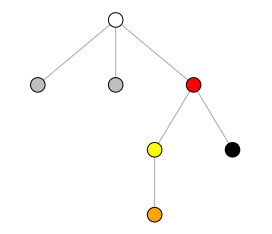
\includegraphics[width=0.2\textwidth]{neighbourhood_time_342}
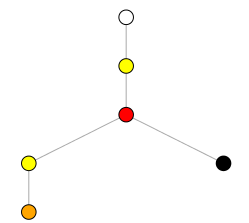
\includegraphics[width=0.19\textwidth]{neighbourhood_time_456}
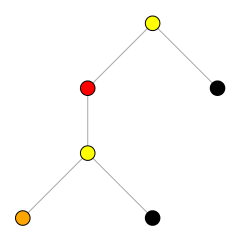
\includegraphics[width=0.18\textwidth]{neighbourhood_time_501}
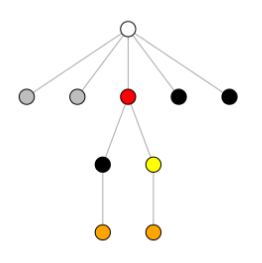
\includegraphics[width=0.18\textwidth]{neighbourhood_time_524}
\caption{Illustration of different real structures using different colors for the root (white), the ego (red) and other posts written by the same author (orange) the ego parent and other posts written by the same author (yellow), posts previous to the ego (grey) and posts posterior to the ego.}
\label{fig:colors}
\end{figure*}

\subsection{Pruning}
At this point, we can still find structures whose only difference is that one of them has more leafs hanging from some of the nodes. Thus, we prune every neighbourhood by leaving a maximum of two consecutive siblings of the same color and where neither of them has any children. The reason of setting the limit to two is that it is the minimum necessary to distinguish between \textit{zero}, \textit{one} and \textit{more than one} consecutive occurrences. In other words, we consider that the difference between one and zero replies to a post is relevant, but that five and six replies do not make any difference worth being represented.    

Figure~\ref{fig:colors} shows some real examples, from our dataset, of time-based neighbourhoods after colouring and pruning.

\section{Application to Reddit forums}
Our data consists of two different forums of Reddit, namely the Podemos dataset \footnote{https://www.reddit.com/r/podemos} and the Game of Thrones dataset\footnote{https://www.reddit.com/r/gameofthrones}. The Podemos forum was conceived in March 2014 as a tool for internal democracy, and forum members used it to debate ideological and organizational principles that were later formalized in their first party congress hold in Madrid the October 18th and 19th 2014. Nowadays, its members use it mainly to share and discuss about political news. The Game of Thrones is a casual discussion forum about the Game of Thrones TV series.
The Podemos dataset contains 75,000 posts corresponding to 4,262 threads written by 9,160 users between the April 25th and October 20th 2014. The Game of Thrones dataset contains 75,000 posts corresponding to 5,862 threads written by 18,907 users.

\subsection{Neighbourhood extraction}
As a previous step for all further analysis we detect the neighbourhood around every post in our datasets. Each neighbourhood structure (including colours) is given a unique integer number. Unfortunately, it is not practical to give a number to every theoretically possible structure since, even if we could enumerate all the possible trees up to a given size, a lot of of these trees would not be seen in the data. It appears then a much more practical approach to enumerate only those trees that are seen in the data. The consequence of this is that every dataset will have its own dictionary of trees. 

We detect the order-based and time-based neighbourhood of every post as follows. A counter for every neighbourhood structure is created the first time it us detected. For every post, we extract its neighbourhood (order-based or time-based) colour and prune it as explained above (Section~\ref{sec:colouring_pruning}). Then we check whether it is isomorphic to some of the already seen neighbourhoods. If this is the case, then we increment the counter for the neighbourhood previously seen. Otherwise we create a new entry for the current neighbourhood. The computational cost of this operation has a upper bound of $\mathcal O(n^2)$, $n$ being the number of posts, for the case where each neighbourhood occurs only once. \footnote{TODO: It's actually much less, probably logarithmic, since the size dictionary grows incrementally}

\subsection{Agreement between neighbourhood methods}
The detection of the time-based and order-based neighbourhood in the Game of Thrones dataset gave us a list of 2000 different (non-isomorphic) time-based neighbourhoods and 180 different (non-isomorphic) \footnote{TODO: Review numbers} order-based neighbourhoods, which means that the time-based is able to capture a much wider set of structures. Of course, this is not necessarily and advantage since these extra structures may be just spurious and only occur a very small number of times. Indeed, Figure~\ref{fig:census_distributions} shows that around half of the time-based neighbourhoods occur only once, and that we only need 384 time-based to cover 95\% of the census, while for the order-based, 53 structures are enough to cover the same percentage. Moreover, there is no much difference, in terms of frequency, between the 50 most frequent neighbours of each type. The reason why the frequency of the order-based neighbourhoods decay faster might be that the most frequent neighbourhood is much more frequent (upper-left red point in the left plot of figure \ref{fig:census_distributions}) than the most frequent time-based neighbourhood.  


The divergent number of neighbourhoods between order-based and times-based brings us to the following question:  how differ the order-based and time-based neighbourhoods given to a same post? We re-labelled the order-based neighbourhoods and assigned them the label of their isomorphic time-based counterparts or the first unused number in the time-based index. This left us a set of 2183 trees. Figure~\ref{fig:confusion} shows, for every post, its time-based neighbourhood and its order-based neighbourhood. Those in the diagonal (34\%) see no difference between the time-based and order-based. Out of the diagonal, there are two rows indicating a high number of posts being assign the same order-based neighbourhood but very different time-based neighbourhoods. These order-based neighbourhoods are the number 1 and the number 50. These collapse of many time-based neighbourhoods into one is significant because it happens a lot among very frequent time-based neighbourhood. In the right plot of Figure ~\ref{fig:confusion} we can see other order-based neighbourhoods that collapse many of the most frequent time-based neighbourhoods, such as the 22, 17, 26, 29, 49, 56, 47 and 101. 


\begin{figure*}
\centering
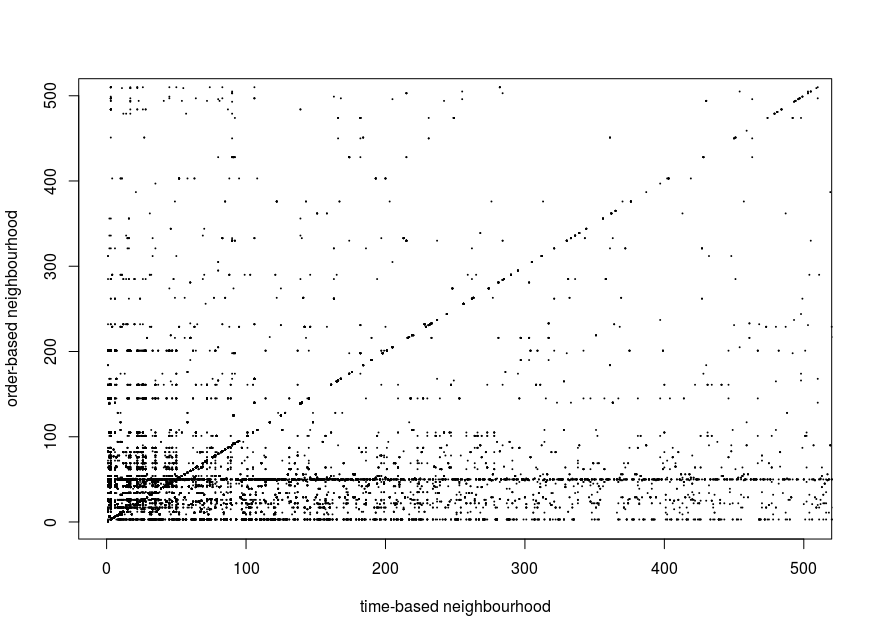
\includegraphics[width=0.5\textwidth]{confusion_time_order_gameofthrones}%
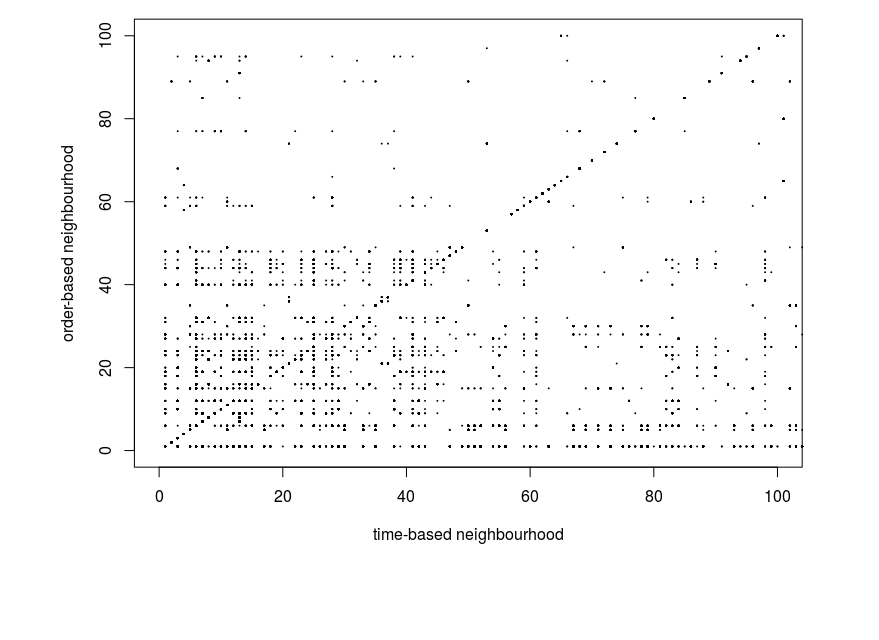
\includegraphics[width=0.5\textwidth]{confusion_time_order_gameofthrones_zoom}
\caption{Neighbourhood of posts from the point of view of order-based and time-based. Neighbourhoods with the same label in the order-based and the time-based axes are isomorphic. The points in the diagonal correspond to posts to whom the two methods assign exactly the same neighbourhood. Horizontal rows of points correspond to posts that are assigned many different time-based neighbourhoods but the same single order-based neighbourhood.}
\label{fig:confusion}
\end{figure*}

\subsection{Neighbourhood census}
Given a set of local structures and a graph under study, a census is a counting of how many times does each structure appear in the graph. In the context of online discussion forums, triad census has been sometimes used in the graph of users interactions are often used (in these graphs, an edge exists from user $u$ to user $v$ if $u$ wrote a post reply to some of the posts written by $v$ in some thread.) \cite{Adamic2008, Lumbreras2013}. However, triads are poor objects when studying trees since there are only three possible structures with, at most, three nodes: a single vertex, a directed dyad (reply), star (two replies to the same post) and a chain (reply and reply to the reply). On the contrary, our neighbourhoods are potentially richer structures that capture the real structure of conversations.

\begin{figure*}
\centering
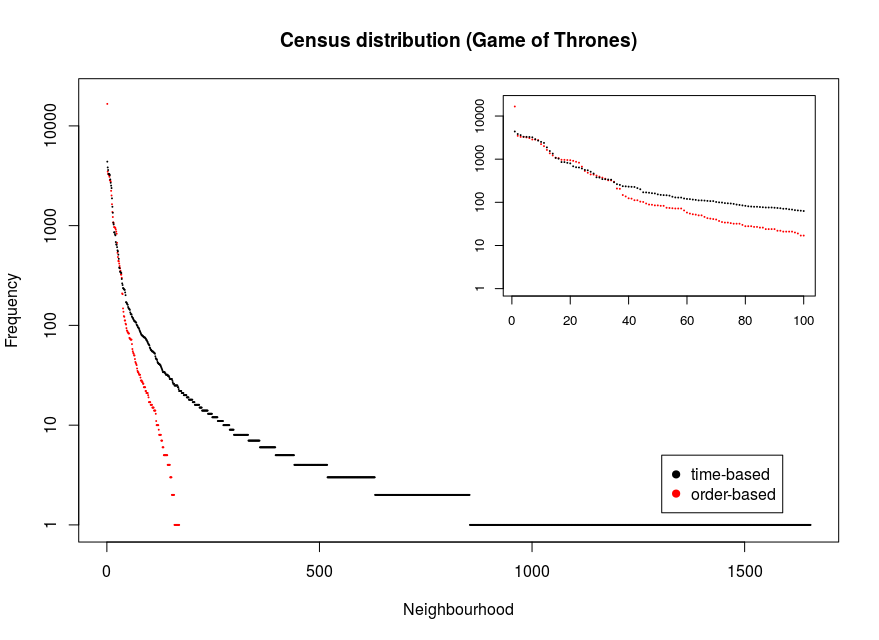
\includegraphics[width=0.5\textwidth]{order_vs_time_census_distribution}%
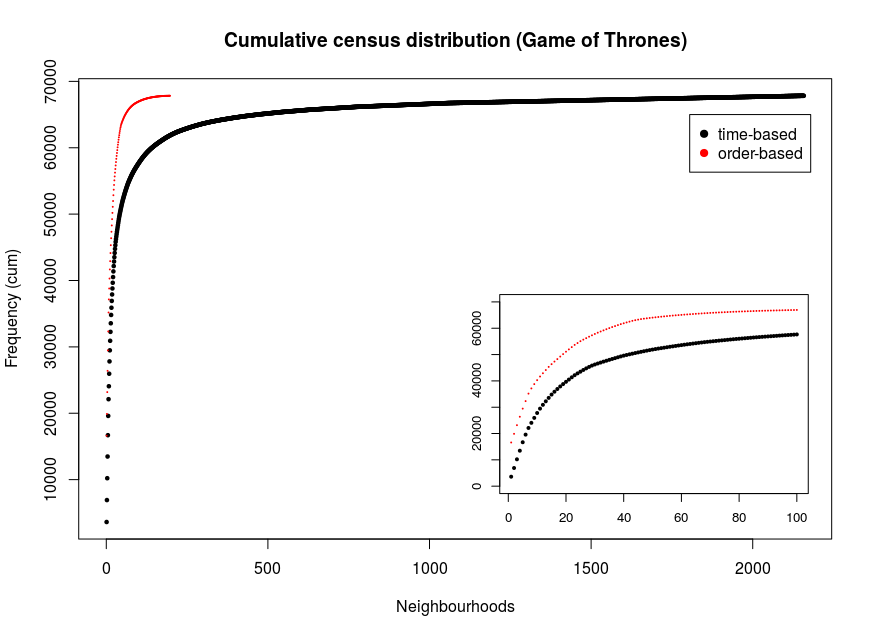
\includegraphics[width=0.5\textwidth]{order_vs_time_census_distribution_cum}
\caption{Comparison of census distributions with order-based and time-based neighbourhoods.}
\label{fig:census_distributions}
\end{figure*}


In Figure \ref{fig:census_compare} we compare the neighbourhood census in the Podemos and the Game of Thrones forums. Interestingly, two time-based neighbourhoods are  more than three times likelier in the Game of Thrones. These neighbourhoods correspond to a discussion between two users (21) and to XXXXXX (25). The same comparison for the order-based triad is harder to interpret, since the outstanding neighbourhoods in the Game of Thrones correspond to XXXX (25) and ... (27)


\begin{figure*}
\centering
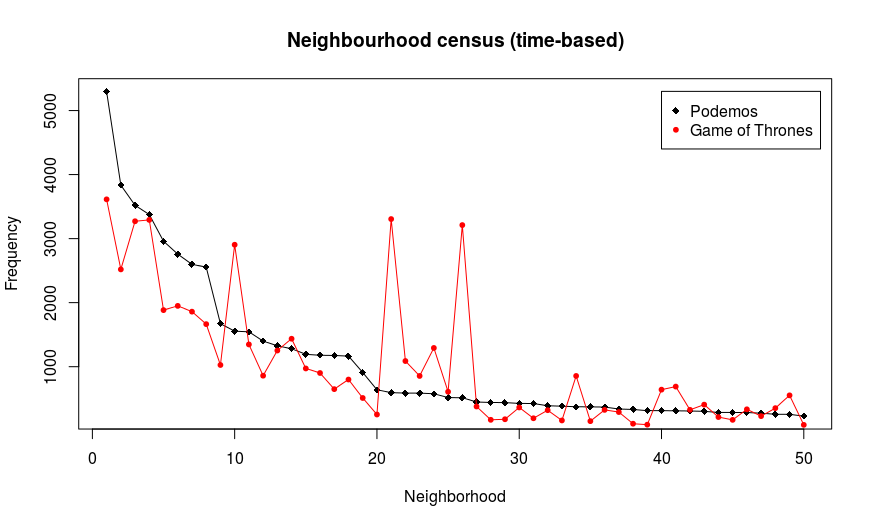
\includegraphics[width=0.5\textwidth]{time_neighbourhood_census_compare_forums}%
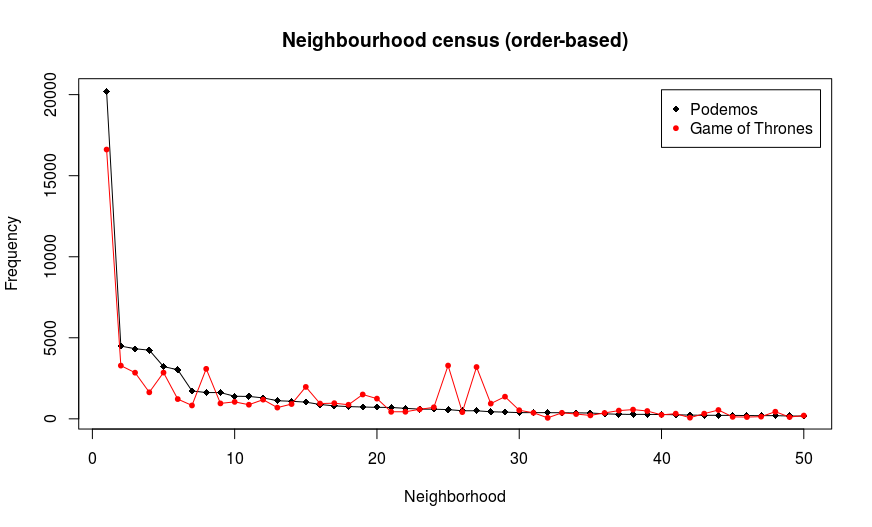
\includegraphics[width=0.5\textwidth]{order_neighbourhood_census_compare_forums}
\caption{Comparison of census for two different forums.}
\label{fig:census_compare}
\end{figure*}

\begin{figure}
\centering
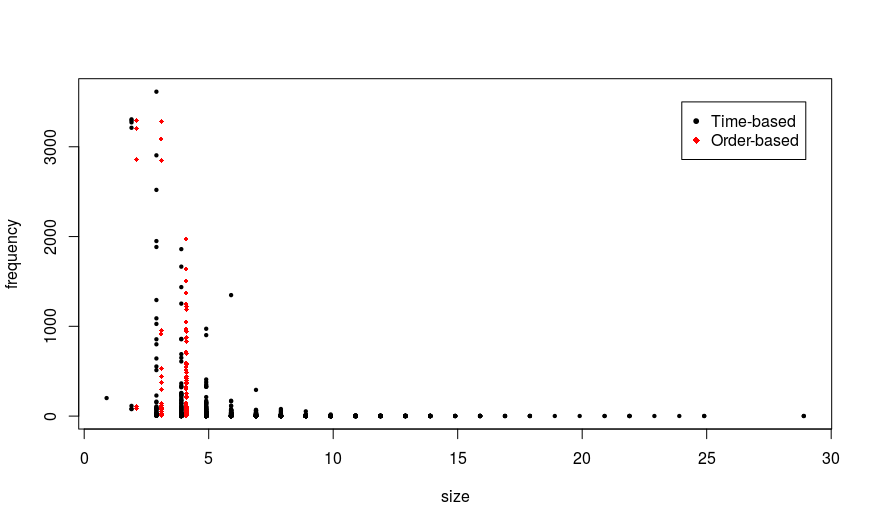
\includegraphics[width=0.5\textwidth]{census_size_vs_freq_gameofthrones}
\caption{Size of neighbourhoods and their frequencies.}
\label{fig:census_size_vs_freq}
\end{figure}


This results lead us to think that the time-based neighbourhood is more convenient than the order-based. The main reason, we think, is that order seems to be a too dogmatic way to decide where a neighbourhood ends.

\subsection{Conversation-based clustering of users}
In this section, we cluster users based on the neighbourhoods of their posts. Our intuition is that some users like participating in some kind of discussion rather than other. Certainly, most part of the information necessary to understand the nature of a discussion in in its textual content. However, due to the huge diversity of topics, vocabulary, and the difficulty of current algorithms to capture the language subtleties such as humour, irony, or context, we turn our attention towards the structure of the discussions, which can also contain some information. We work under the  hypothesis that the structural-neighbourhoods in which a user post in embedded reflect the kind of conversation in that part of the thread. 

We limit our study to a set of 100 \textit{active users} who wrote more than 100 posts. For those users, we create an initial feature matrix $U\times N$ where $U$ is the number of users and $N$ is the number of neighbourhoods in the census, and where the the position $(u,n)$ is a counter of the number of times that a post written by user $u$ has a neighbourhood isomorphic to $n$. We drop those feature columns that are zero for every user (these are neighbourhoods seen only around posts of users with low-level activity). To make the feature vector of a user independent on the number of posts, we transform the counts into percentages. And since some features have much higher percentages than others for most users, we scale and normalize the matrix so that every feature has mean 0 and variance 1. To avoid non-significant scores, we remove also the feature column corresponding to neighbourhoods that have a frequency less than 50 among the active users.

We use k-means to find the clusters, though one can use any other clustering method. Since the plot over the Within-Cluster Sum of Squares for $k=1,...20$ did not show any clear elbow we chose $k=3$ clusters so that clusters are easier to interpret. We did the clustering over a feature matrix with order-based neighbourhoods and another feature matrix with time-based neighbourhoods. Figure~\ref{fig:PCA} and shows the PCA projections of the users coloured by their assigned cluster. 

\begin{figure}
	\centering
	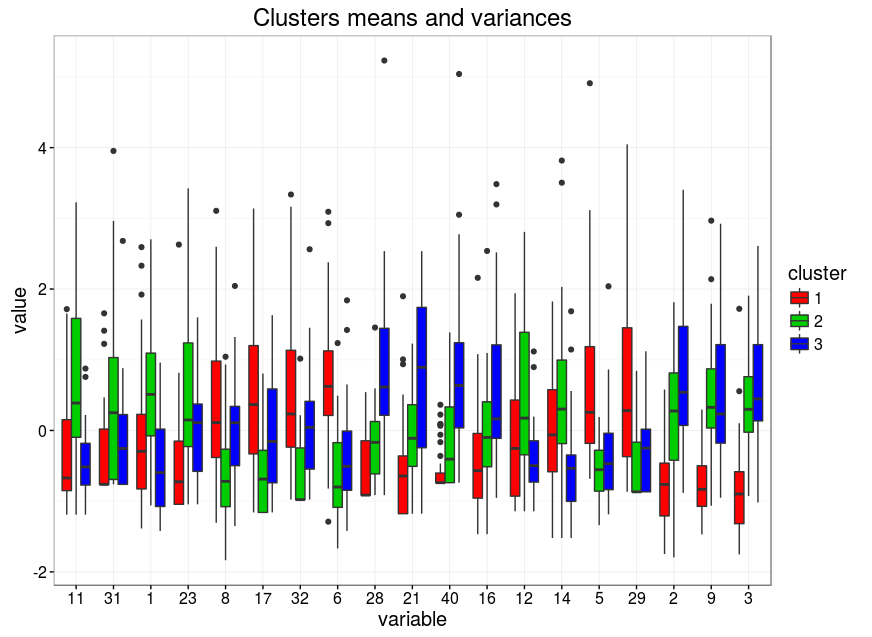
\includegraphics[width=0.5\textwidth]{whiskers}
	\caption{Whiskers plots in the most relevant features (time-based)}
	\label{fig:PCA}
\end{figure}

% TODO: Paragraph to explain similarity between clusters assignments

% TODO: Paragraph to explain which motifs are prefered for every cluster

% TODO: paragraph discussing a visual/manual analysis of some users

\begin{figure*}
	\centering
	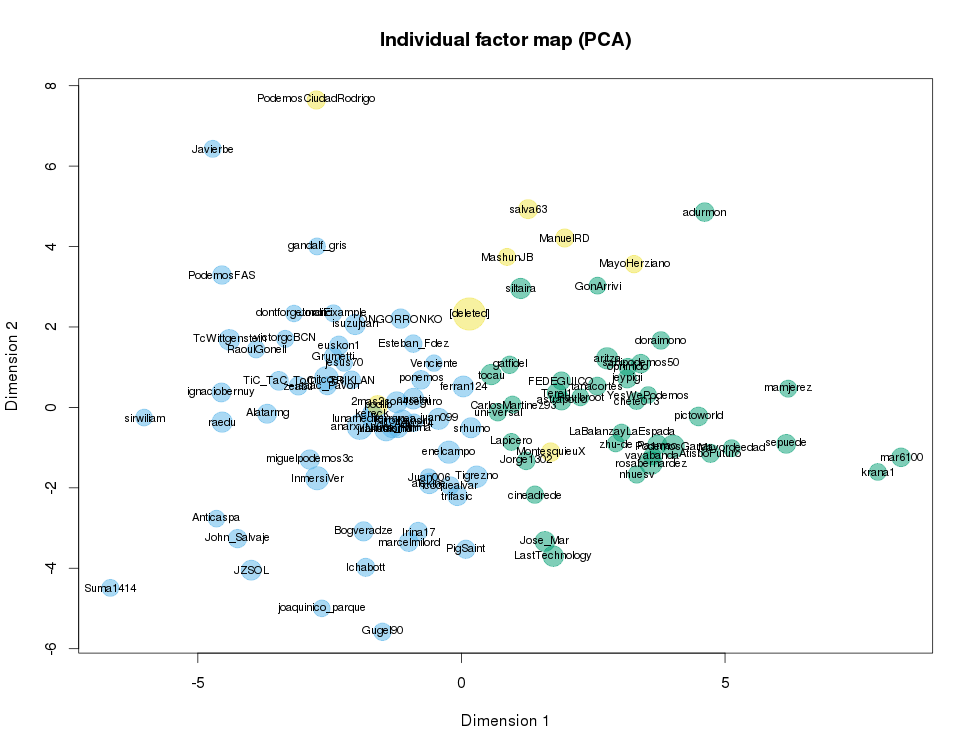
\includegraphics[width=0.9\textwidth]{PCA_cluster_orderbased}
	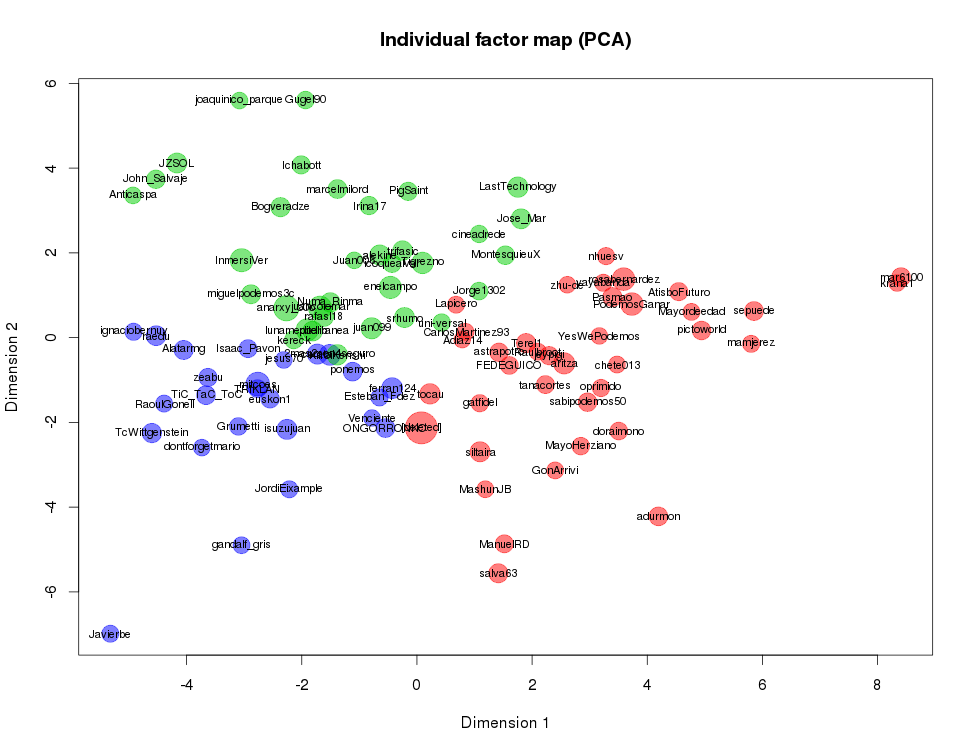
\includegraphics[width=0.9\textwidth]{PCA_cluster_timebased}
	\caption{PCA projections of the order-based (above) and time-based (below) neighbourhood features}
	\label{fig:PCA}
\end{figure*}

%Interpretation


% Maybe mention that we can take for instance only the posts before the ego and use it to understand when when can recommend a post based on the structure.

\section{Conclusions}
We presented a method to characterise conversations of users in online threads. Due to the tree nature of online threads, traditional patters such as triads are not able to capture much of relevant dynamics of a conversation. Our defined order-based and temporal-based neighbourhoods 
are able to capture a very rich variety of structures. We used this neighbourhoods to characterise users in terms of the structure of the conversations they participate in and showed that, indeed, there are different types of structural conversationalists

%Future
The concept of structural-temporal neighbourhood opens the door to some interesting paths of research. One might wonder whether other pruning are more pertinent than the proposed here. Also, even after pruning some neighbourhoods suggest the same type of conversation, so a manual merge might be convenient. Maybe sociologists can help to merge the found neighbourhoods in a meaningful way.   

% use section* for acknowledgment
%\section*{Acknowledgment}

% trigger a \newpage just before the given reference
% number - used to balance the columns on the last page
% adjust value as needed - may need to be readjusted if
% the document is modified later
%\IEEEtriggeratref{8}
% The "triggered" command can be changed if desired:
%\IEEEtriggercmd{\enlargethispage{-5in}}


\bibliographystyle{IEEEtran}
\bibliography{bibliography}
\newpage
\section*{Appendix}
\begin{figure*}
	\centering
	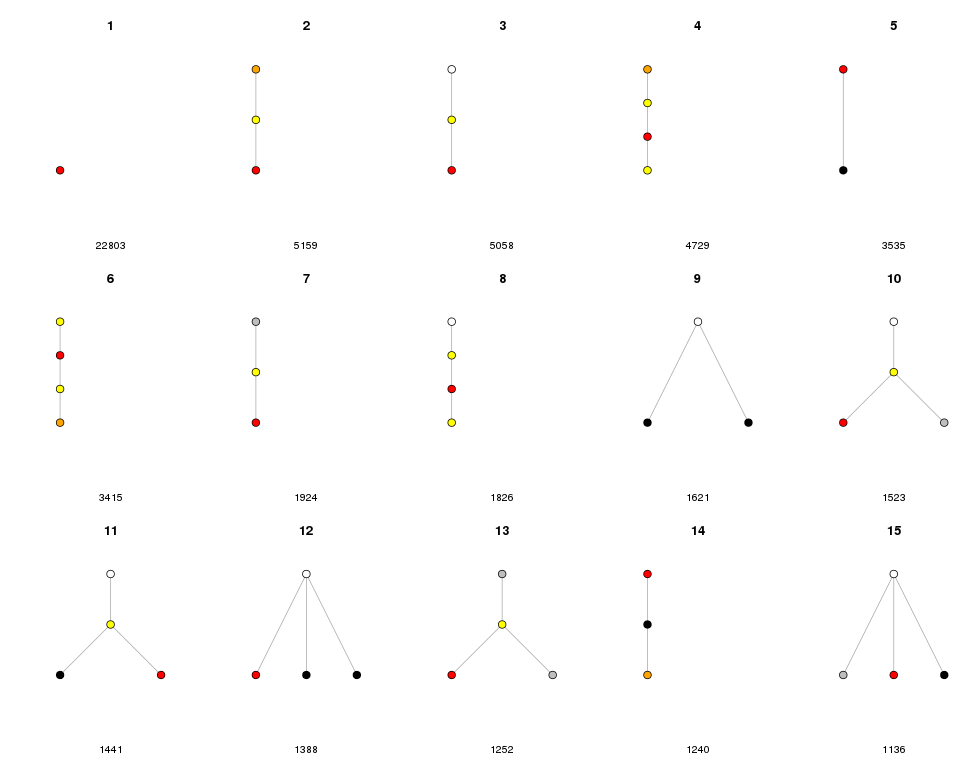
\includegraphics[width=0.8\textwidth]{census_orderbased_1}
	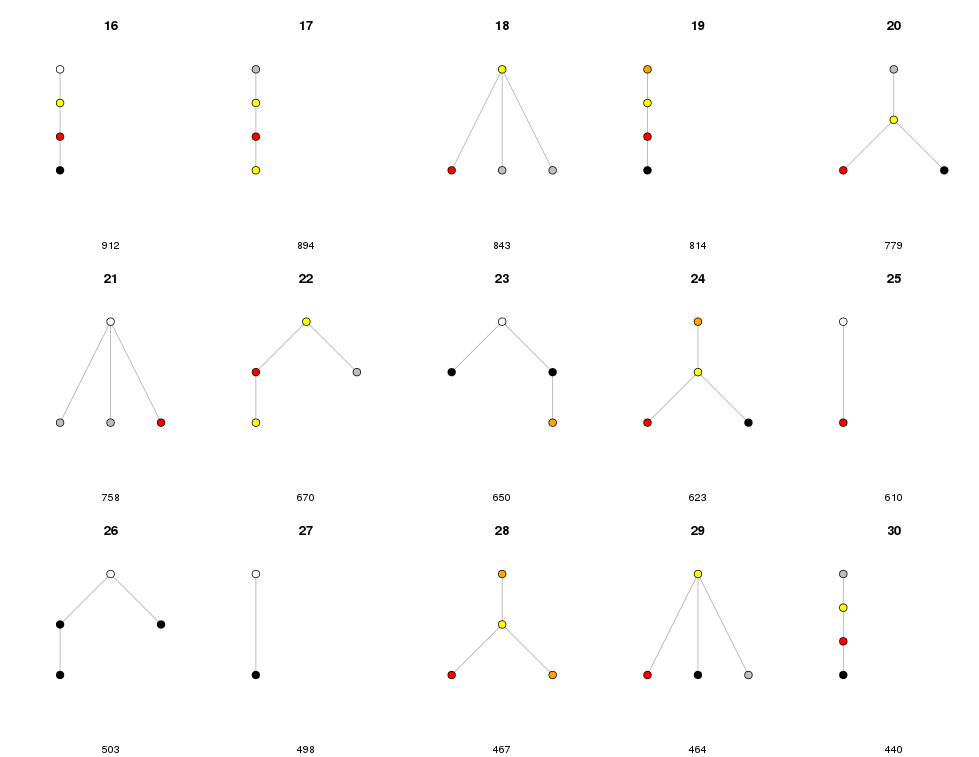
\includegraphics[width=0.8\textwidth]{census_orderbased_2}
	%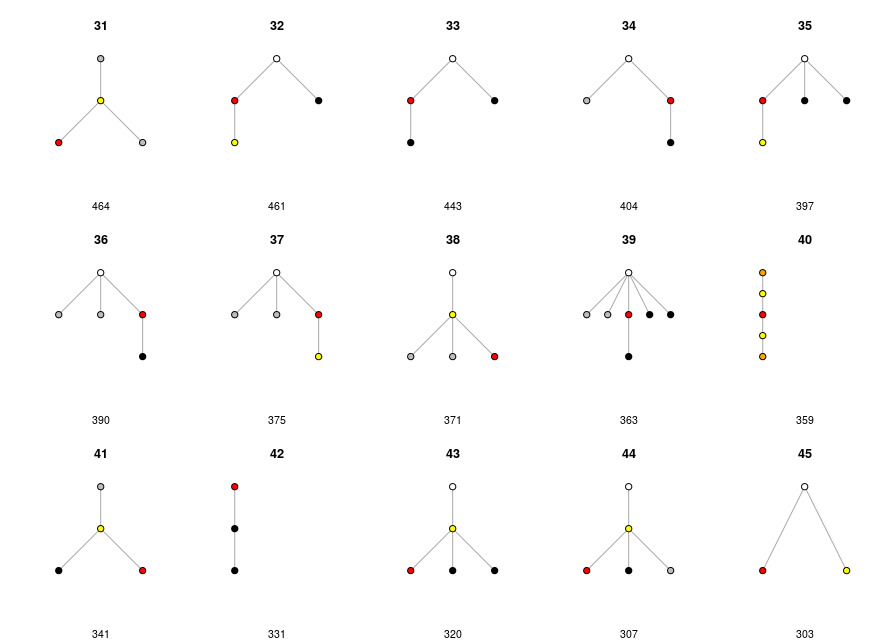
\includegraphics[width=0.75\textwidth]{census_orderbased_3}
	\caption{Most frequent order-based neighbourhoods with $r=2$ and $n=4$ (Podemos)}
	\label{fig:census_orderbased}
\end{figure*}
\begin{figure*}
	\centering
	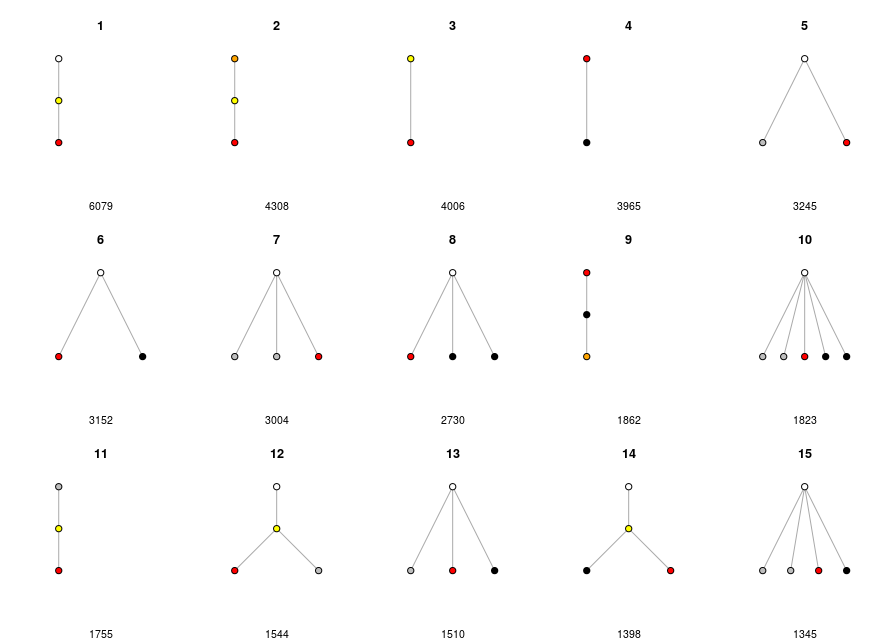
\includegraphics[width=0.8\textwidth]{census_timebased_1}
	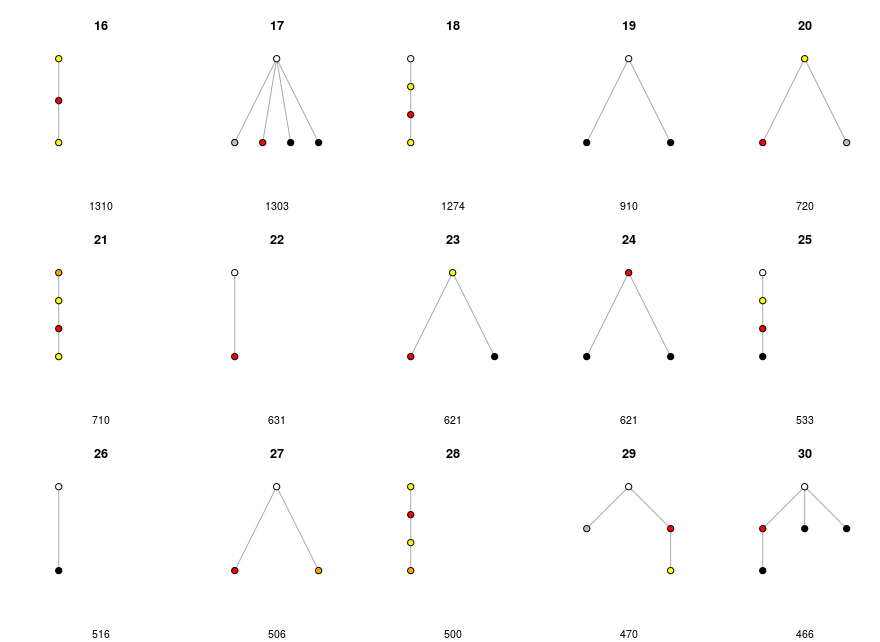
\includegraphics[width=0.8\textwidth]{census_timebased_2}
	%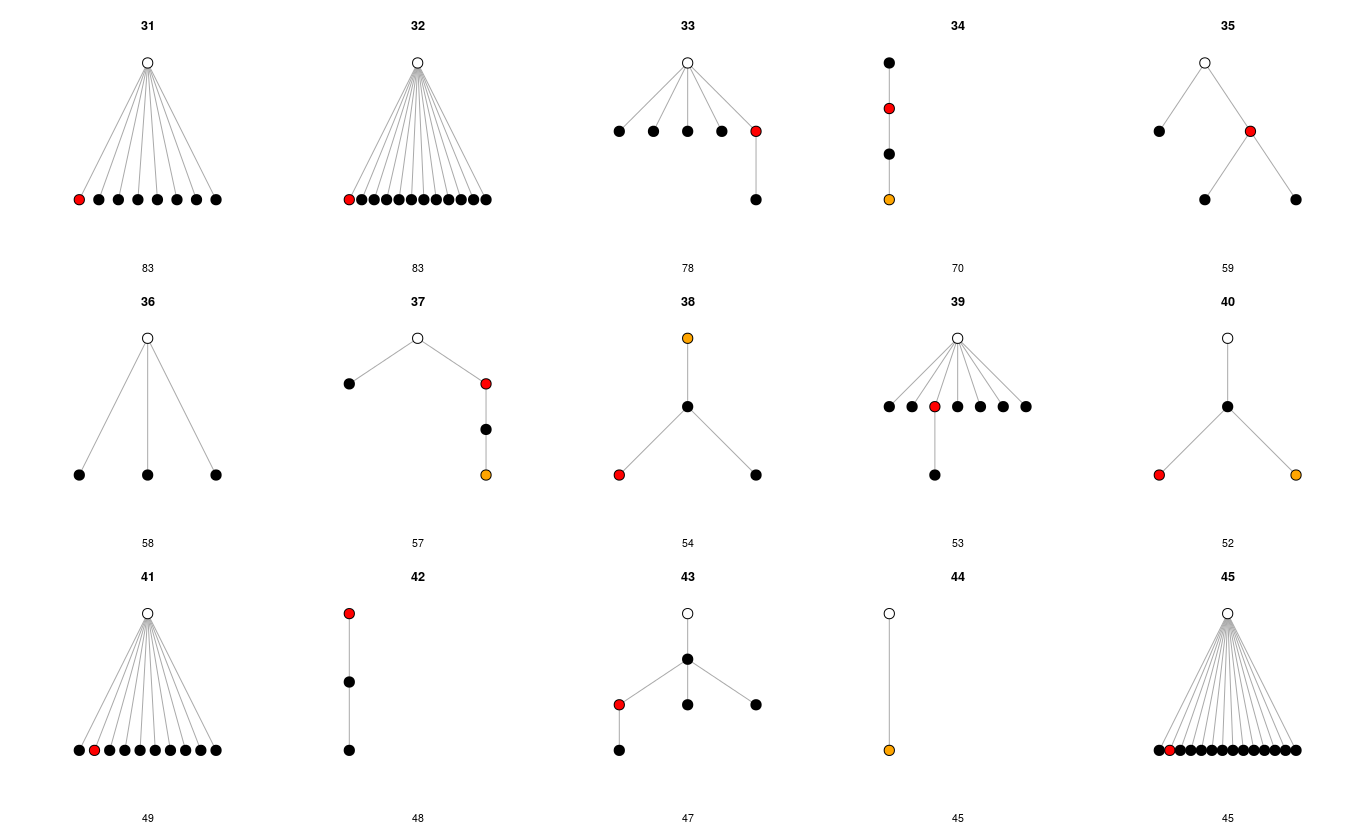
\includegraphics[width=0.8\textwidth]{neighbourhoods_time_3}
	\caption{Most frequent time-based neighbourhoods (Podemos)}
	\label{fig:neighbourhoods_time}
\end{figure*}

\begin{figure*}
\centering
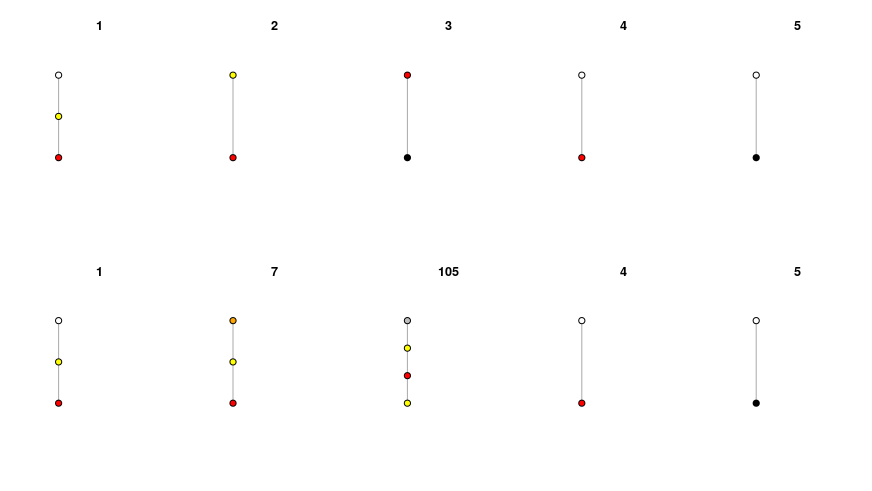
\includegraphics[width=1\textwidth]{confusion_time_order_motifs_gameofthrones_1}
\caption{Most popular time-based neighbourhoods (up) and how they are mostly detected in order-based neighbourhood (down).}
\label{fig:census_size_vs_freq}
\end{figure*}


% that's all folks
\end{document}


